% ------------------------------------------------------------------------ %
% !TEX encoding = UTF-8
% !TEX TS-program = pdflatex
% !TEX root = ../Project.tex
% !TEX spellcheck = en-EN
% ------------------------------------------------------------------------ %
%
% ------------------------------------------------------------------------ %
% 	CHAPTER TITLE
% ------------------------------------------------------------------------ %
%
\chapter{Requirements Traceability}
%
\label{cap:requirementstraceability}
%
%
Providing traceability of system requirements to design components is important for determining
if and how system requirements have been realised. The RTM (Requirements Traceability Matrix)
also is needed to understand if all design components are necessary and to quickly understand
the impact of changing a requirement. Non Functional requirements are detailed more in general in the other parts of the document. 
The matrix displays Functional requirements on the rows (check RASD for more deatils on section 3.A) and the components needed to satisfy these Functional Requirements on the columns.

\begin{landscape}
\begin{center}
\thispagestyle{empty}
\makebox[\textwidth][c]{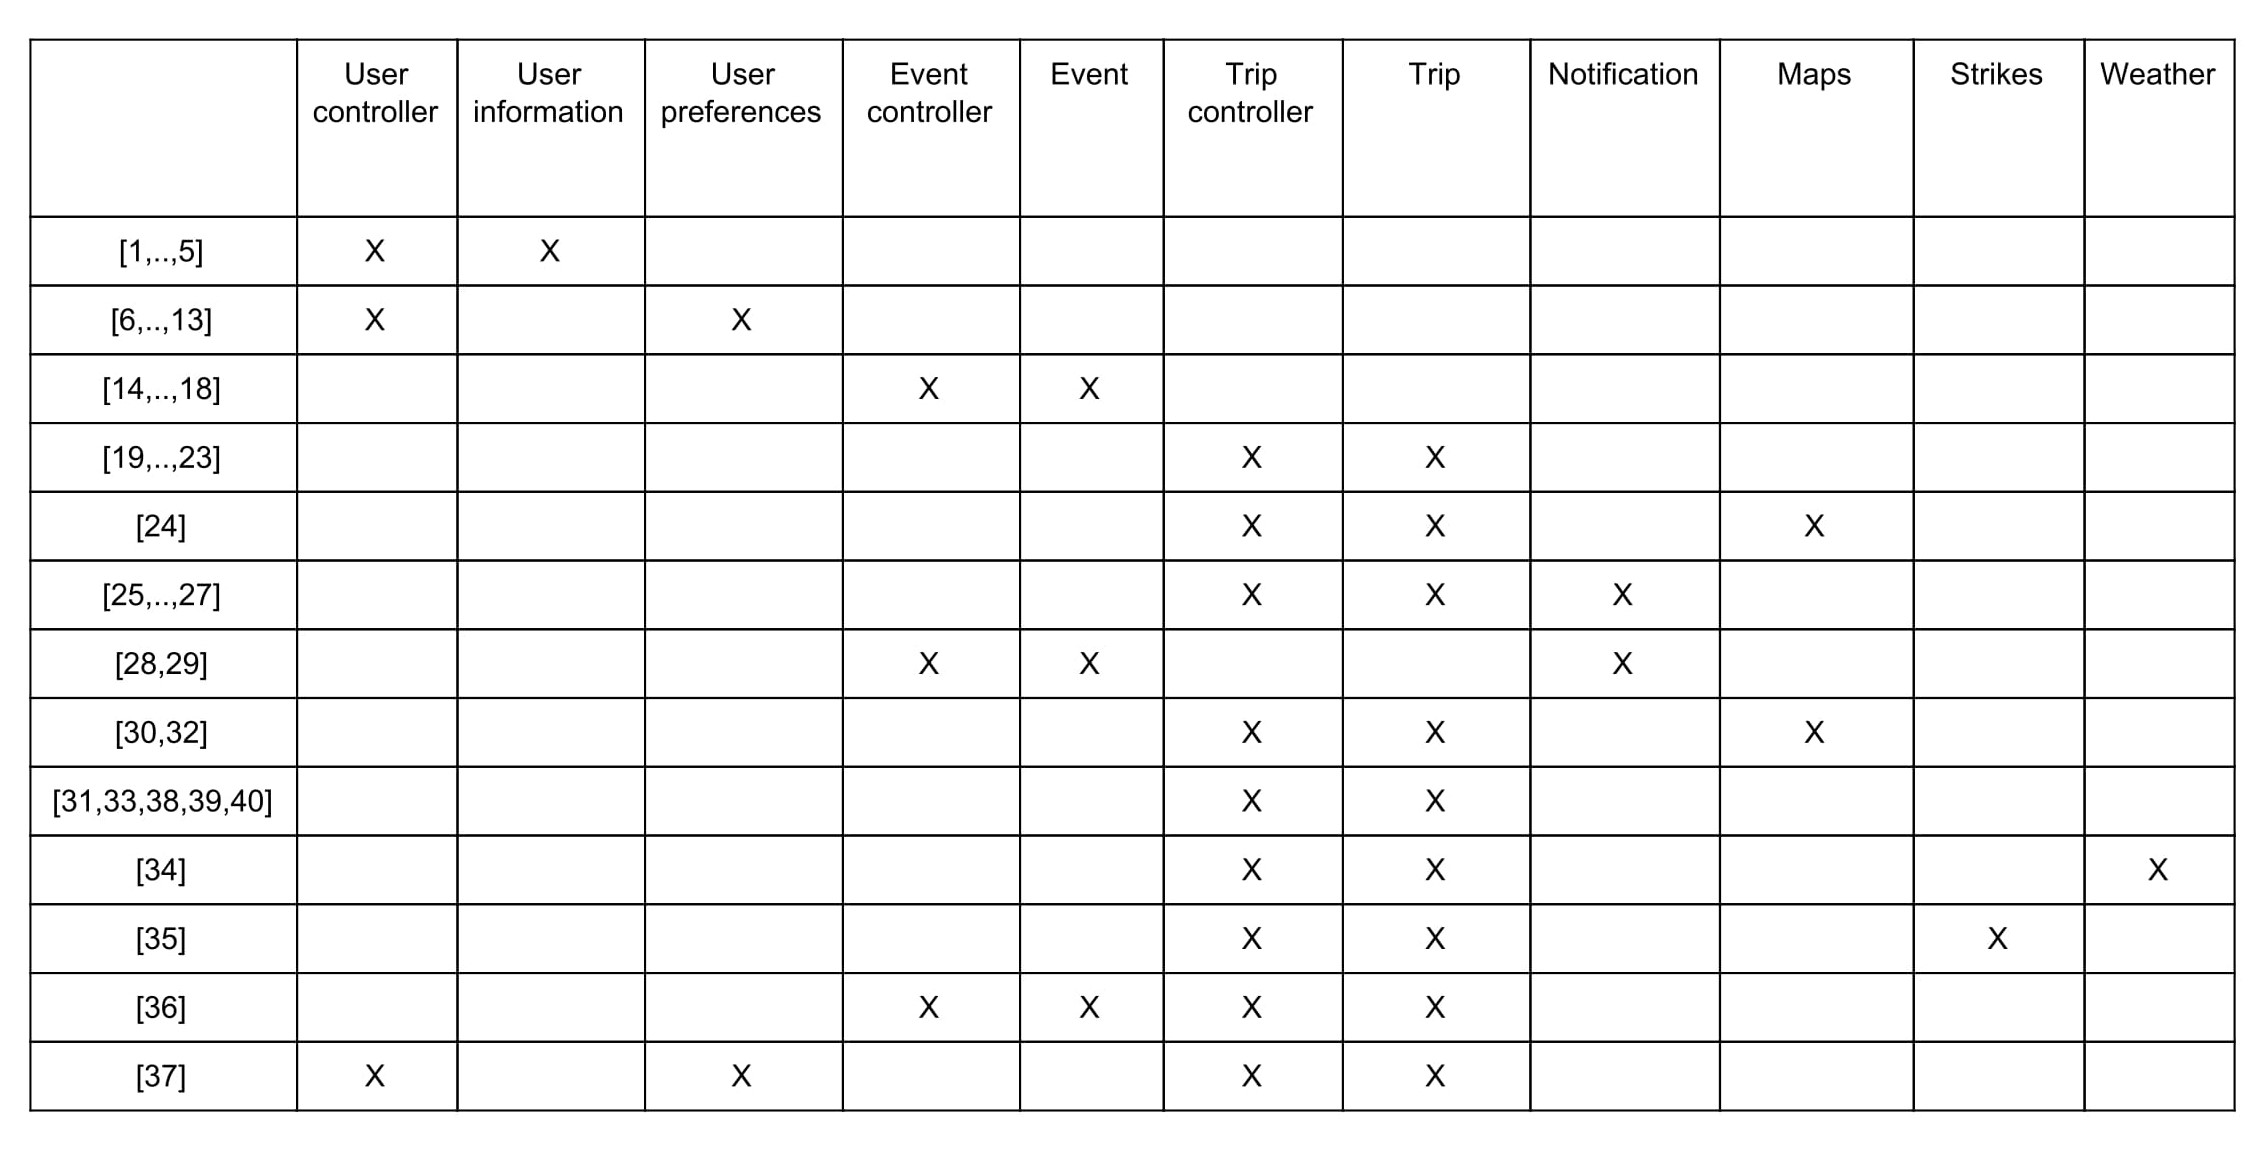
\includegraphics[width=1.8\textwidth]{MainMatter/images/req/table}}
\captionof{figure}{Requirements Traceability Matrix}
\end{center}
\end{landscape}

% -----------------------------END------------------------------------- %
